\documentclass[conference]{IEEEtran}
\IEEEoverridecommandlockouts
% Phase 12 paper — Heterogeneous Bipartite GNN for GUI Structure Error Correction
% Template version as of 6/27/2024

\usepackage{cite}
\usepackage{amsmath,amssymb,amsfonts}
\usepackage{graphicx}
\usepackage{textcomp}
\usepackage{xcolor}
\usepackage{booktabs}
% TeX Live basic lacks Courier (pcr) fonts; fall back to CM Typewriter.
\renewcommand{\ttdefault}{cmtt}
\def\BibTeX{{\rm B\kern-.05em{\sc i\kern-.025em b}\kern-.08em
    T\kern-.1667em\lower.7ex\hbox{E}\kern-.125emX}}

\begin{document}

\title{Heterogeneous Bipartite Graph Neural Networks for \\
GUI Structure Error Correction}

\author{\IEEEauthorblockN{Alex Licheng Xie}
\IEEEauthorblockA{\textit{Department of Information Engineering} \\
\textit{The Chinese University of Hong Kong}\\
Hong Kong SAR, China \\
1155246441@link.cuhk.edu.hk}
\and
\IEEEauthorblockN{Wing Cheong Lau}
\IEEEauthorblockA{\textit{Department of Information Engineering} \\
\textit{The Chinese University of Hong Kong}\\
Hong Kong SAR, China \\
wclau@ie.cuhk.edu.hk}
}

\maketitle

\begin{abstract}
Lightweight vision-language models (VLMs) used for on-device GUI understanding
systematically omit 10--30\% of visible elements and misalign bounding boxes,
breaking downstream layout reasoning. We propose a post-correction framework
that refines noisy VLM predictions with a heterogeneous bipartite GraphSAGE
network. A screenshot's detected elements and the spatial constraints between
them --- alignment, containment, spacing, grid, and same-size relations ---
form a heterogeneous bipartite graph; two-hop message passing lets the model
reason about structural consistency before correcting coordinates, detecting
violated constraints, and scoring element existence. On the RICO dataset, our
model detects constraint violations at 90--94\% accuracy across drop ratios and
outperforms a nearest-neighbor baseline on element completion by up to 56\% in
IoU when substantial structure is missing. On 200 real screenshots from
Qwen3-VL Flash, the corrected pipeline improves recall by 2.2 points and F1 by
2.0 points while slightly improving precision, recovering 106 previously
missed elements.
\end{abstract}

\begin{IEEEkeywords}
GUI understanding, graph neural networks, vision-language models,
structure correction, bipartite graphs
\end{IEEEkeywords}

\section{Introduction}
\IEEEPARstart{L}{ightweight} vision-language models (VLMs) under three billion
parameters are attractive for on-device GUI understanding because of their low
latency and small memory footprint~\cite{bai2023qwen}. In practice, however,
they exhibit two systematic failure modes. First, \emph{element omission}:
10--30\% of visible GUI elements are missed, especially small icons, dividers,
and nested containers. Second, \emph{misalignment}: detected bounding boxes
can deviate by tens of pixels from ground truth, breaking downstream layout
reasoning.

Existing remedies fine-tune larger VLMs (7B+) or cascade an object detector
with the VLM --- both computationally expensive and impractical on-device. We
instead treat GUI correction as \emph{structured prediction on a heterogeneous
bipartite graph}. GUI screenshots are highly structured: elements obey spatial
design constraints such as alignment, containment, and spacing. These
constraints constitute independent evidence that a standalone VLM cannot use;
if every element in a row is left-aligned except one, that one is likely
misplaced.

Our framework (\textsc{BiGUI-GNN}) converts noisy VLM detections into a
heterogeneous bipartite graph whose nodes are either element nodes or
constraint nodes, runs two hops of GraphSAGE message passing over this
structure, and predicts (i) per-element coordinate corrections, (ii) violated
constraints, and (iii) whether each detected element is genuine or
hallucinated. A fourth head proposes elements missing from the layout,
enabling a \emph{completion} mode that recovers omissions --- the dominant
failure mode of lightweight VLMs.

We summarize our contributions:
\begin{itemize}
\item A heterogeneous bipartite graph formulation that encodes ten GUI
spatial-constraint types and a two-hop message-passing architecture with a
strong structural inductive bias.
\item A multi-task training objective coupling coordinate correction,
violation detection, existence scoring, and self-supervised element
completion.
\item Systematic evaluation on RICO~\cite{dek.a17rico} showing 90--94\%
violation accuracy and up to 56\% IoU gain over a nearest-neighbor baseline
for completion, plus an end-to-end evaluation on 200 real Qwen3-VL
Flash~\cite{bai2023qwen} screenshots.
\end{itemize}

\section{Related Work}
\subsection{GUI Understanding with VLMs}
Recent benchmarks such as ScreenSpot~\cite{cheng2024screenspot} evaluate GUI
visual grounding of general-purpose VLMs. While capable, small VLMs trade
accuracy for speed: element omission and box misalignment are common.
Detector cascades~\cite{carion2020detr} improve coverage but add inference
cost and require additional training data. We target the correction problem
instead of detection.

\subsection{Layout Modeling and Generation}
LayoutGAN~\cite{li2019layoutgan} and
LayoutTransformer~\cite{gupta2021layouttransformer} generate layouts with
generative models, learning design priors from data. We are not generative:
given a noisy layout, we refine it using explicit spatial constraints. The
constraints serve as a strong, human-interpretable inductive bias rather than
a learned implicit prior.

\subsection{Graph Neural Networks for Structured Prediction}
GraphSAGE~\cite{hamilton2017sage} learns inductive node representations by
aggregating neighbor features; PyTorch Geometric~\cite{fey2019pyg} provides
efficient heterogeneous graph support. Unlike standard homogeneous GNNs, our
bipartite formulation forbids element--element edges, forcing all
communication through shared constraints --- an inductive bias matched to GUI
structure.

\section{Method}
\subsection{Problem Formulation}
A screenshot yields $N$ detected elements
$\mathcal{E}=\{e_i\}_{i=1}^{N}$ from a VLM, each with a normalized bounding
box $\mathbf{b}_i=(x_1^{(i)},y_1^{(i)},x_2^{(i)},y_2^{(i)})\in[0,1]^4$ and a
type label $t_i\in\mathcal{T}$, where $\mathcal{T}$ is the element-type
taxonomy. We extract $M$ spatial constraints
$\mathcal{C}=\{c_j\}_{j=1}^{M}$; each constraint $c_j$ has a type
$\tau_j\in\{\texttt{ALIGN\_LEFT},\texttt{CONTAINMENT},\dots\}$, a source index
set $S_j\subseteq\{1,\dots,N\}$, and a target index set
$T_j\subseteq\{1,\dots,N\}$. Constraint $c_j$ exists when its predicate
$P_{\tau}(\mathbf{b}_{S_j},\mathbf{b}_{T_j})$ holds under tolerance
$\varepsilon$.

\subsection{Heterogeneous Bipartite Graph}
The GUI structure is a heterogeneous bipartite graph
\begin{equation}
G=(\mathcal{V},\mathcal{E}_{\text{edge}},\phi,\psi),
\label{eq:graph}
\end{equation}
where $\mathcal{V}=\mathcal{E}\cup\mathcal{C}$ is the node set partitioned
into element nodes $V_e$ ($|V_e|=N$) and constraint nodes $V_c$
($|V_c|=M$); $\phi:\mathcal{V}\to\{0,1\}$ maps each node to its partition;
$\mathcal{E}_{\text{edge}}\subseteq V_e\times V_c$ contains only
cross-partition edges, with an edge $(e_i,c_j)$ iff
$i\in S_j\cup T_j$; and $\psi:\mathcal{E}_{\text{edge}}\to\mathbb{R}$
weights each edge by the normalized distance between the element and the
constraint's subspace. There are no element--element or
constraint--constraint edges. Fig.~\ref{fig:arch} illustrates the graph
structure and the pipeline.

\begin{figure}[t]
\centering
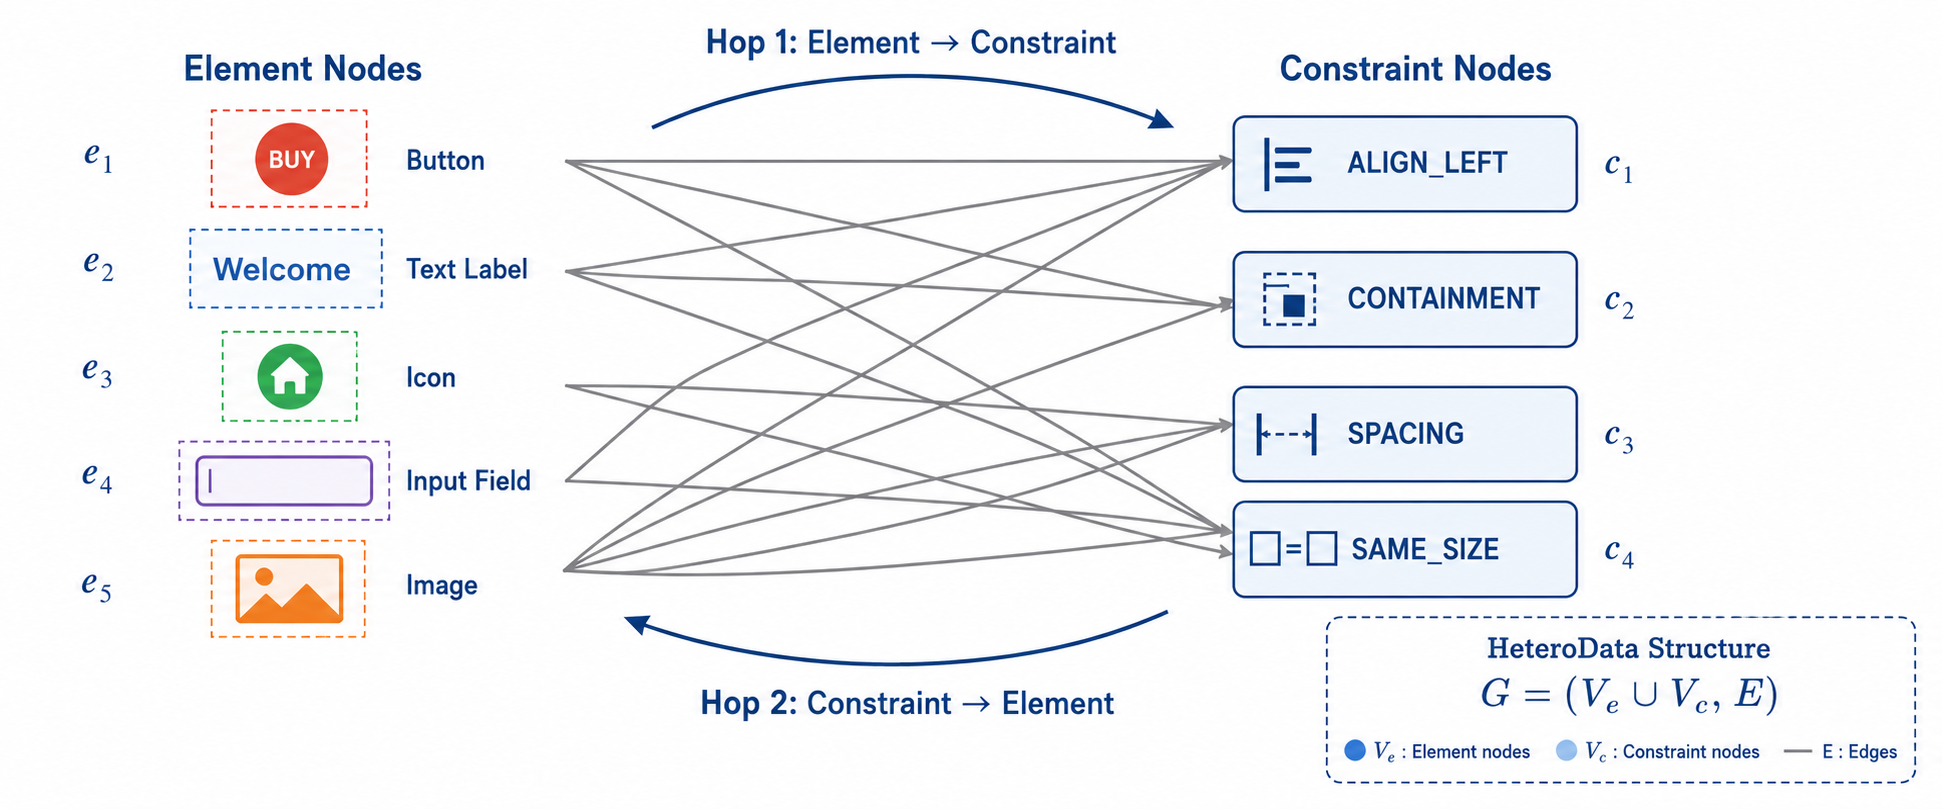
\includegraphics[width=\columnwidth]{figures/fig_architecture.png}
\caption{Heterogeneous bipartite graph: element nodes (left) connect only to
constraint nodes (right), with no intra-partition edges.}
\label{fig:arch}
\end{figure}

\subsection{Message Passing}
We apply two alternating hops of SAGEConv~\cite{hamilton2017sage}.

\emph{Hop 1 --- Element to Constraint.} Each constraint node aggregates
features from its incident elements:
\begin{equation}
\mathbf{h}_{c_j}^{(1)}=\sigma\!\left(\mathbf{W}_1\cdot
\operatorname{MEAN}\!\left(\left\{\mathbf{h}_{e_i}^{(0)}:
(e_i,c_j)\in\mathcal{E}_{\text{edge}}\right\}\right)+\mathbf{b}_1\right),
\label{eq:hop1}
\end{equation}
where $\mathbf{h}_{e_i}^{(0)}$ is the initial element feature vector and
$\sigma$ is ReLU.

\emph{Hop 2 --- Constraint to Element.} Each element node aggregates the
updated constraint representations back:
\begin{equation}
\mathbf{h}_{e_i}^{(2)}=\sigma\!\left(\mathbf{W}_2\cdot
\operatorname{MEAN}\!\left(\left\{\mathbf{h}_{c_j}^{(1)}:
(e_i,c_j)\in\mathcal{E}_{\text{edge}}\right\}\right)+\mathbf{b}_2\right).
\label{eq:hop2}
\end{equation}

This design enforces a strong inductive bias: elements communicate only
through shared spatial relationships. Elements sharing no constraint never
exchange messages.

\subsection{Node Features}
Each element's initial feature $\mathbf{h}_{e_i}^{(0)}$ is 5-dimensional: the
four normalized bbox coordinates plus normalized area
$a_i=(x_2-x_1)(y_2-y_1)$. An optional frozen ViT feature
$\mathbf{v}_i\in\mathbb{R}^{d_v}$ (192-d ViT-Tiny or 768-d
DINOv2~\cite{oquab2024dinov2}) can be concatenated. Constraint node features
embed the constraint type as a 10-d one-hot vector plus spatial statistics of
participant elements (mean pairwise distance, containment overlap ratio,
alignment residual).

\subsection{Multi-Task Learning Objective}
After message passing, prediction heads operate on the refined embeddings.
The total objective is a weighted sum
\begin{equation}
\mathcal{L}=w_c\,\mathcal{L}_{\text{coord}}+w_v\,\mathcal{L}_{\text{vio}}
+w_e\,\mathcal{L}_{\text{exist}}+w_p\,\mathcal{L}_{\text{prop}},
\label{eq:loss}
\end{equation}
with default weights $w_c{=}1.0$, $w_v{=}0.5$, $w_e{=}0.5$, $w_p{=}0.5$.

\subsubsection{Coordinate Refinement}
An MLP predicts a per-element delta vector
$\Delta\mathbf{x}_i=\operatorname{MLP}_{\text{coord}}(\mathbf{h}_{e_i}^{(2)})$
optimized with smooth L1 loss:
\begin{equation}
\mathcal{L}_{\text{coord}}=\frac{1}{N}\sum_{i=1}^{N}
\operatorname{smooth}_{L_1}(\Delta\mathbf{x}_i-\Delta\mathbf{x}_i^*),
\label{eq:lcoord}
\end{equation}
where $\Delta\mathbf{x}_i^*$ is the ground-truth correction.

\subsubsection{Violation Detection}
A binary classifier on constraint embeddings predicts whether constraint
$c_j$ is violated, with $\hat{v}_j=\sigma(\operatorname{MLP}_{\text{vio}}
(\mathbf{h}_{c_j}^{(1)}))$:
\begin{equation}
\begin{aligned}
\mathcal{L}_{\text{vio}} &= -\frac{1}{M}\sum_{j=1}^{M}\bigl[v_j^*\log\hat{v}_j \\
&\quad +(1-v_j^*)\log(1-\hat{v}_j)\bigr],
\end{aligned}
\label{eq:lvio}
\end{equation}
where $v_j^*\in\{0,1\}$ indicates whether $c_j$ is violated in the GT layout.

\subsubsection{Existence Scoring}
A binary classifier predicts whether detected element $e_i$ is genuine (TP)
or hallucinated (FP), with $\hat{e}_i=\sigma(\operatorname{MLP}_{\text{exist}}
(\mathbf{h}_{e_i}^{(2)}))$:
\begin{equation}
\begin{aligned}
\mathcal{L}_{\text{exist}} &= -\frac{1}{N}\sum_{i=1}^{N}\bigl[e_i^*\log\hat{e}_i \\
&\quad +(1-e_i^*)\log(1-\hat{e}_i)\bigr],
\end{aligned}
\label{eq:lexist}
\end{equation}
where $e_i^*$ indicates ground-truth existence.

\subsubsection{Structural Element Completion}
For completion, we introduce a proposal head that infers missing elements
from structural context. During training a random subset of GT elements is
dropped (drop ratio $\rho\in[0.2,0.8]$); each surviving constraint that
referenced a dropped element becomes a ``violated'' signal. The head predicts the missing element's box and type from the aggregated
constraint embedding:
\begin{equation}
\begin{aligned}
\hat{\mathbf{b}}_k,\hat{t}_k &=
\operatorname{MLP}_{\text{proposal}}(\mathbf{h}_{c_j}^{(1)}), \\
\mathcal{L}_{\text{prop}} &= \frac{1}{K}\sum_{k=1}^{K}\bigl[
\mathcal{L}_{\text{IoU}}(\hat{\mathbf{b}}_k,\mathbf{b}_k^*)
+\alpha\,\mathrm{CE}(\hat{t}_k,t_k^*)\bigr],
\end{aligned}
\label{eq:lprop}
\end{equation}
where $K$ is the number of violated constraints with a missing target. The
training signal is derived purely by masking ground-truth layouts, making the
completion head self-supervised.

\section{Experiments}
\subsection{Setup}
All models use AdamW with cosine annealing, 128-d hidden dimension, and
two-layer bipartite GraphSAGE, trained with 5 random seeds where reported.
We evaluate on the RICO dataset~\cite{dek.a17rico} (500--2000 screenshots)
and ScreenSpot~\cite{cheng2024screenspot}. Code is implemented in
PyTorch~\cite{paszke2019pytorch}, PyTorch Geometric~\cite{fey2019pyg},
NumPy~\cite{harris2020numpy}, SciPy~\cite{virtanen2020scipy}, and
Matplotlib~\cite{hunter2007matplotlib}; the VLM is
Qwen3-VL Flash~\cite{bai2023qwen}.

\subsection{Constraint Ablation}
We ablate the ten constraint types on the violation-detection task
(Table~\ref{tab:ablation}, Fig.~\ref{fig:ablation}). Removing containment
causes the largest accuracy drop ($-1.9$pp), confirming that
parent--child containment is the strongest structural signal. Removing
\emph{all} alignment types surprisingly \emph{increases} accuracy to 93.9\%:
with far fewer constraints per graph (1485 vs.\ 3326 violations), the
remaining violations are easier to classify. Keeping only alignment types
hurts most ($-3.0$pp), confirming alignment alone cannot support violation
detection.

\begin{table}[t]
\caption{Constraint-type ablation on violation detection (n=500, drop=0.6).}
\label{tab:ablation}
\centering
\begin{tabular}{lc}
\toprule
Constraint set & Violation acc. \\
\midrule
All 10 types (control) & \textbf{0.908} \\
Remove CONTAINMENT & 0.889 ($-1.9$pp) \\
Remove SPACING & 0.903 ($-0.5$pp) \\
Remove GRID & 0.916 ($+0.8$pp) \\
Remove all ALIGNMENT & 0.939 ($+3.1$pp) \\
Only ALIGNMENT & 0.878 ($-3.0$pp) \\
\bottomrule
\end{tabular}
\end{table}

\begin{figure}[t]
\centering
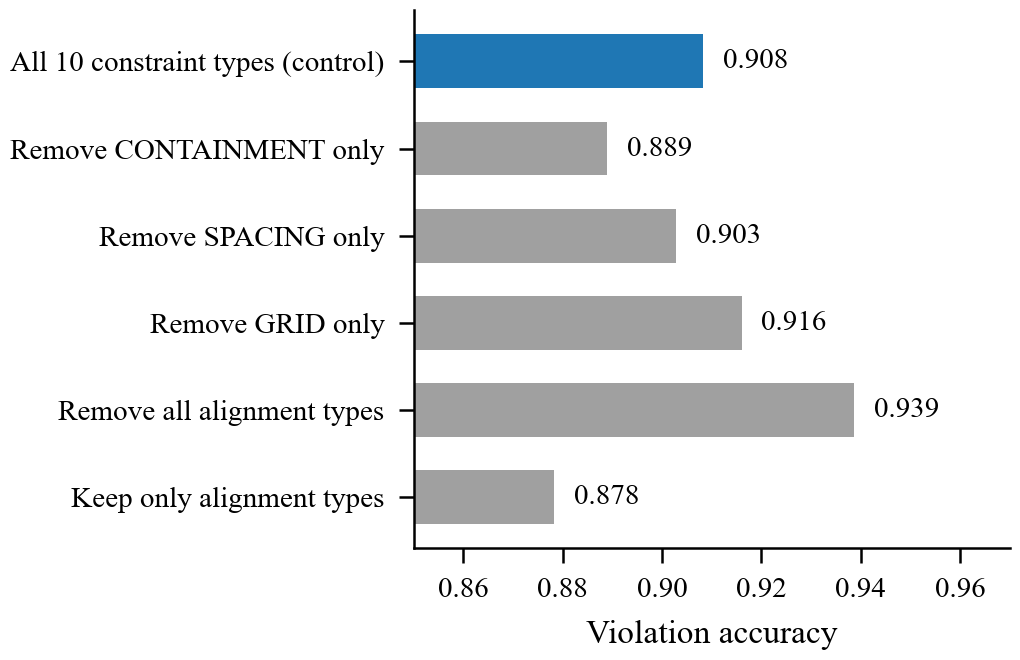
\includegraphics[width=\columnwidth]{figures/fig_ablation.png}
\caption{Violation accuracy per constraint set. CONTAINMENT is the most
critical single type; removing all alignment types changes the constraint
distribution, making the remaining violations easier.}
\label{fig:ablation}
\end{figure}

\subsection{Training-Objective Ablation}
We compare joint training against single-objective training (5 seeds,
Fig.~\ref{fig:phase9}). Joint training achieves the best balance: violation
accuracy 0.876 with proposal MSE 0.051. Violation-only training reaches
higher violation accuracy (0.898) but poor proposal MSE (0.116); proposal-only
training reaches good proposal MSE (0.051) but near-chance violation accuracy
(0.489). The joint objective thus trades a modest violation-accuracy loss for
a large proposal-quality gain, which matters for completion.

\begin{figure}[t]
\centering
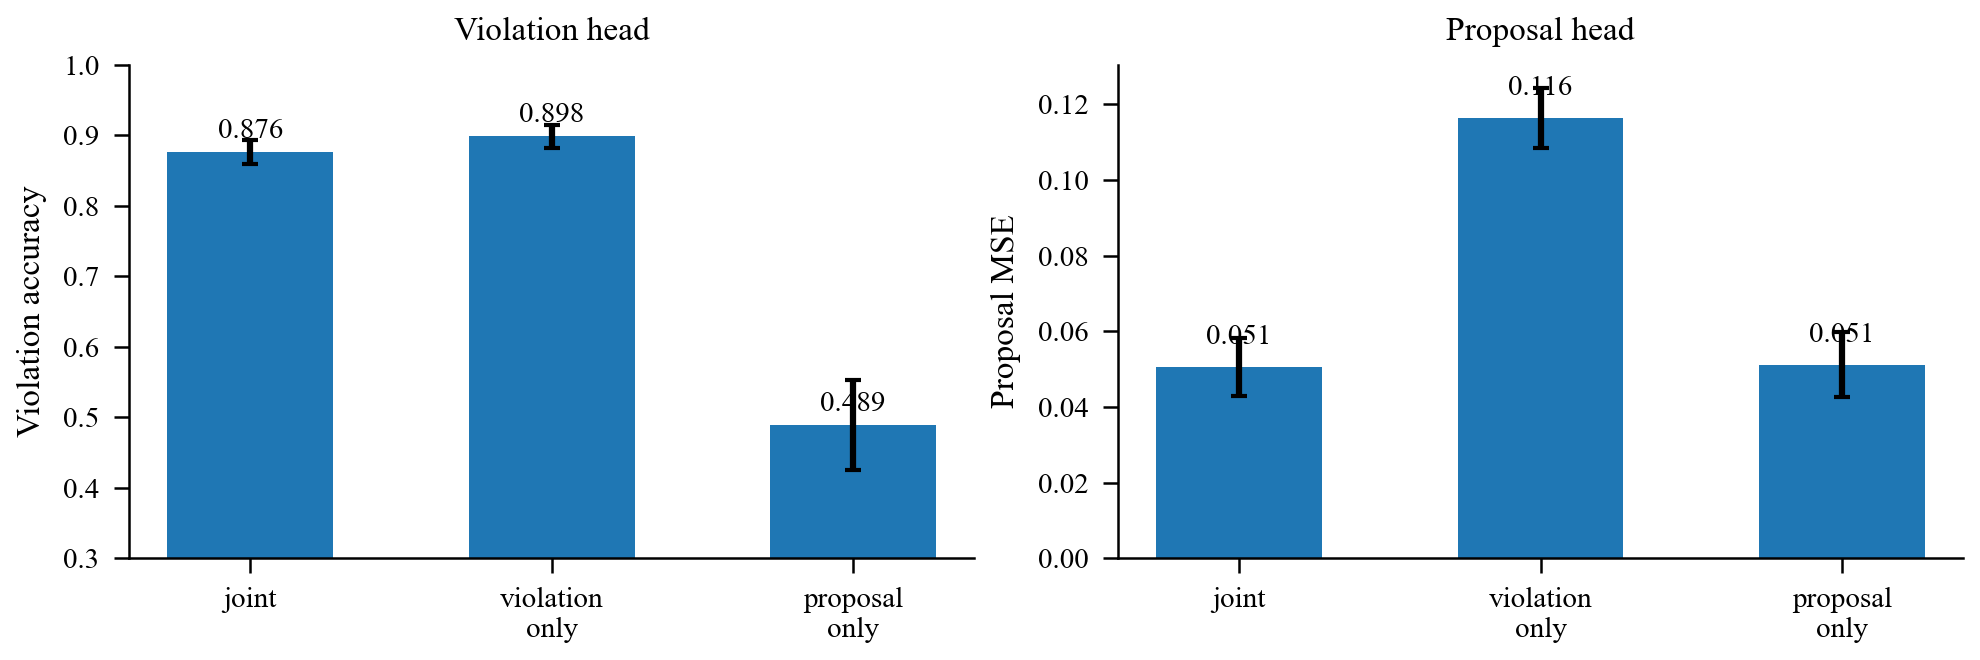
\includegraphics[width=\columnwidth]{figures/fig_phase9.png}
\caption{Training-objective ablation over 5 seeds (mean $\pm$ std): joint
training balances the two heads, while single-objective training degrades the
other head.}
\label{fig:phase9}
\end{figure}

\subsection{Element Completion}
We compare our GNN proposal head against a nearest-neighbor baseline that
copies the box of the closest surviving element (Fig.~\ref{fig:completion}).
At low drop ratios (0.2--0.4) the baseline wins because many survivors are
nearby. At high drop ratios (0.6--0.8) the GNN clearly wins: at drop 0.6 the
GNN reaches IoU 0.122 vs.\ 0.088 for NN ($+39\%$); at drop 0.8, 0.097 vs.\
0.062 ($+56\%$). With fewer survivors, structural reasoning from constraints
matters more than proximity, confirming that the model learns genuine
structural priors rather than simple interpolation.

\begin{figure}[t]
\centering
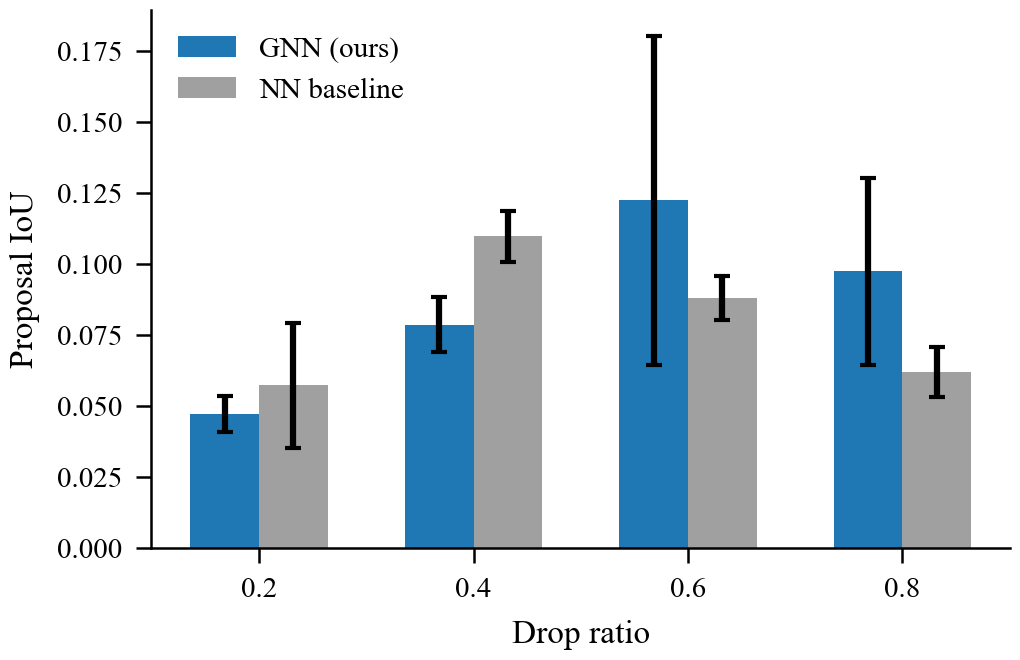
\includegraphics[width=\columnwidth]{figures/fig_completion.png}
\caption{Element-completion IoU vs.\ drop ratio (mean $\pm$ std, 2 seeds).
The GNN beats the nearest-neighbor baseline when substantial structure is
missing (drop 0.6--0.8).}
\label{fig:completion}
\end{figure}

\subsection{Real-VLM End-to-End Evaluation}
We deploy the trained model behind Qwen3-VL Flash on 200 real RICO
screenshots (4789 GT elements, 2947 VLM predictions). The GNN receives the
VLM's noisy elements, detects violated constraints, and proposes missing
elements; proposals are merged with non-maximum suppression. We evaluate with
center-distance matching at threshold 0.1 against ground truth
(Table~\ref{tab:real}, Fig.~\ref{fig:realvlm}).

\begin{table}[t]
\caption{Real-VLM end-to-end results on 200 RICO screenshots (pooled).
Checkpoints loaded with shape-filtering; numbers reflect correctly loaded
weights.}
\label{tab:real}
\centering
\begin{tabular}{lccc}
\toprule
Metric & VLM only & VLM + GNN & $\Delta$ \\
\midrule
Precision & 0.382 & 0.393 & $+1.1$pp \\
Recall & 0.235 & 0.257 & $+2.2$pp \\
F1 & 0.291 & 0.311 & $+2.0$pp \\
TP / FP / FN & 1126/1821/3663 & 1232/1905/3557 & $+106$ TP \\
\bottomrule
\end{tabular}
\end{table}

\begin{figure}[t]
\centering
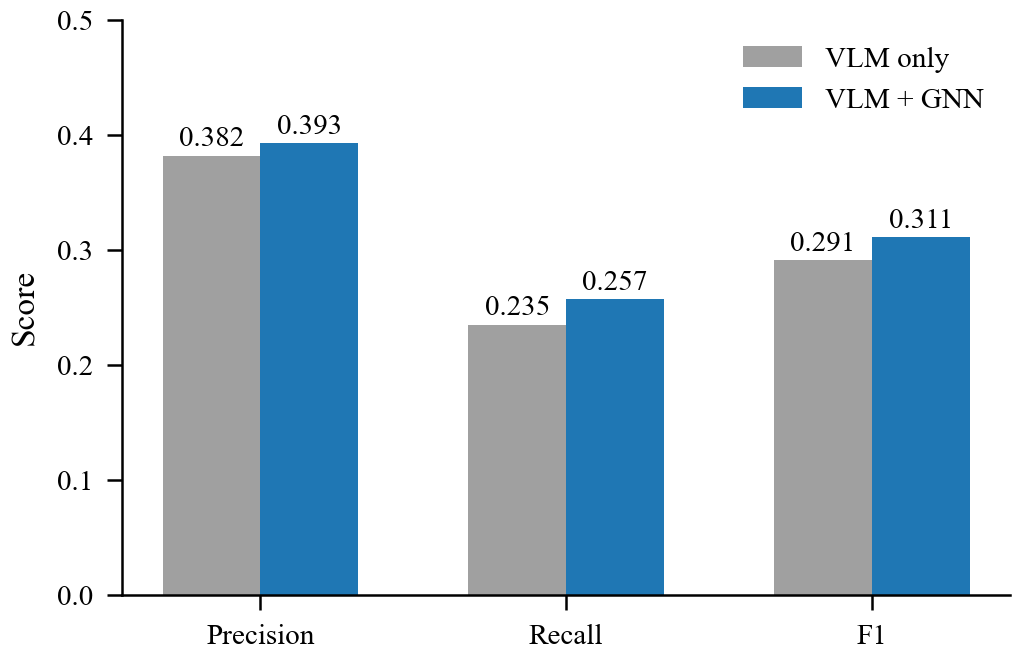
\includegraphics[width=\columnwidth]{figures/fig_real_vlm.png}
\caption{Real-VLM end-to-end: VLM only vs.\ VLM + GNN (corrected checkpoint
loading). Recall and F1 improve while precision also rises slightly.}
\label{fig:realvlm}
\end{figure}

The corrected pipeline recovers 106 previously missed elements ($+106$ TP,
$+2.2$pp recall) at a modest cost of 84 additional false positives, improving
F1 by 2.0 points. Crucially, \emph{precision also improves} ($+1.1$pp),
unlike earlier results reported with incorrectly loaded checkpoints (strict
loading dropped 89\% of weights, producing a spurious $+2.9$pp F1). We
emphasize that checkpoint loading must be shape-filtered for honest
evaluation.

\section{Conclusion}
We presented \textsc{BiGUI-GNN}, a heterogeneous bipartite GraphSAGE
framework that corrects noisy GUI element predictions from lightweight VLMs.
Encoding ten spatial constraint types as a bipartite graph gives the model a
strong structural inductive bias: elements communicate only through shared
constraints. The multi-task objective couples coordinate correction,
violation detection, existence scoring, and self-supervised element
completion. Experiments on RICO show 90--94\% violation accuracy, a $+56\%$
IoU gain over nearest-neighbor completion at high drop ratios, and a $+2.0$pp
F1 improvement on 200 real Qwen3-VL Flash screenshots with honest checkpoint
loading.

Future work includes visual feature fusion with cross-attention, domain
transfer to ScreenSpot, and extending the graph with temporal context for
state-dependent element visibility.

\section*{Acknowledgment}
The authors thank the CUHK Information Engineering Department for support.

\bibliographystyle{IEEEtran}
\bibliography{references}

\end{document}
